\documentclass[margin=1mm]{standalone}
\usepackage{tikz}

\begin{document}
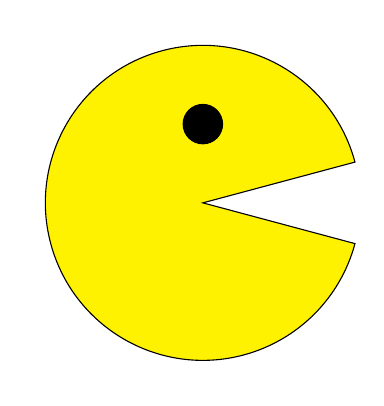
\begin{tikzpicture}
	
	\def\startangle{30};
	\def\endangle{60};
	\def\raio{3};
	
	
	\def\raiopac{2.00};
    
    \def \anglepac{15};

	\pgfmathparse{\raiopac*cos(\anglepac)}
	\edef\xi{\pgfmathresult}
		
	\pgfmathparse{\raiopac*sin(\anglepac)}
	\edef\yi{\pgfmathresult}
    
	\filldraw[fill opacity=1,fill=yellow] (0,0) -- (\xi,\yi) arc (\anglepac:360-\anglepac:\raiopac cm) -- cycle;
	
	\filldraw[fill opacity=1,fill=black] (0.25,1) arc (0:360:0.25 cm) -- cycle;

	
\end{tikzpicture}
\end{document}
